%!TEX root = Slic3r-Manual.tex

\subsection{Speeding Things Up} % (fold)
\label{sec:speeding_things_up}
\index{speed}

Once the printer is reliably producing good quality prints it may be desirable to increase the speed.  Doing this provides several benefits, the most obvious of which is that the results are produced quicker, but also faster print times can be utilised in producing more layers, i.e. lower layer height, thus improving perceived print quality.  An additional benefit is that a faster travel movement, between extrusions, can reduce the effects of oozing.

The best approach is to increment the various speed parameters in small steps and observe the effect each change has on print quality.  Travel speed is a safe starting point, and it is not unrealistic to attain speeds of up to 250mm/s (if your printer can handle it).  Adjusting the speed of perimeters, infill is available in simple mode, and the general rule is to have the perimeter go a little slower than the infill in order to reduce possible blemishes on the surface (infill can be faster because slight gaps will not matter as much).

Expert mode offers more parameters to fine tune printer speeds.  Differentiation between external, small and other perimeters, infill locations, and bridges and gaps are available, as well as the ability to slow down for the first layer.

\begin{figure}[H]
\centering
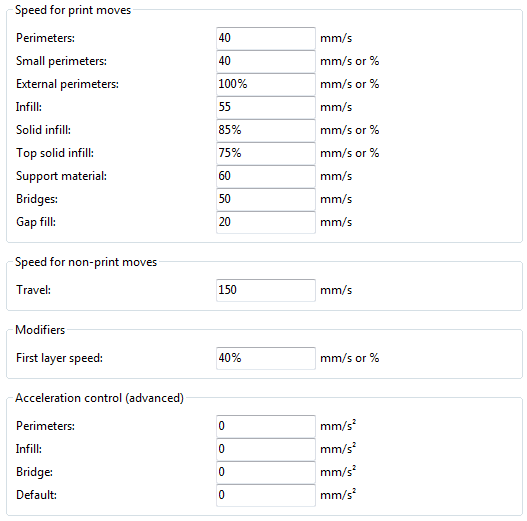
\includegraphics[keepaspectratio=true,width=0.75\textwidth]{tuning/speed_advanced_settings.png}
\caption{Expert mode speed options.}
\label{fig:speed_advanced_settings}
\end{figure}

Where indicated a value can be given in percentage.  This is in relation to the preceding value, e.g. 50\% solid infill would be half of the value defined for infill.

A few general guidelines for each option:
\begin{itemize}
	\item \texttt{Perimeters}  - In expert mode this parameter can be increased slightly as the \texttt{External perimeters} option can be used to ensure blemish free external faces.
	\item \texttt{Small perimeters}  - Meant for holes, islands and fine details, a slower speed here is recommended.
	\item \texttt{External perimeters}  - A slightly slower value may ensure cleaner surfaces.
	\item \texttt{Infill}  - As fast as you can without compromising the integrity of the fill structure.  Faster extrusions can break and result in weak spots.
	\item \texttt{Solid infill}  - The bottom of the model, and any additional solid layers is usually slightly slower than infill but faster than perimeters.
	\item \texttt{Top solid infill}  - Allow time for the extrusion to cleanly cover the previous top layers and result in a tidy top surface.  the last few layers should have bridged the infill structure nicely, preparing the way for a neat finish. 
	\item \texttt{Support material}  - Generally support structures are quick and dirty, and so long as the base is adequately supported they can be built as quickly as they can.
	\item \texttt{Bridges}  - Having the extrusion span distances depends on the material and cooling.  Going too slow will result in sagging, too fast will result in broken strands.  Experimentation is the key here, but generally bridging runs slower than perimeters.
	\item \texttt{Gap fill}  - Filling in small gaps results in the extruder quickly oscillating and the resulting shaking and resonance could have a detrimental affect on the printer.  A smaller value here can guard against this. 
	\item \texttt{Travel}  - As fast as your printer will allow in order to minimise ooze.
	\item \texttt{First layer speed}  - As mentioned in section \ref{sec:the_important_first_layer}, the first layer is important to lay down correctly, and a slower pace helps enormously.  Setting a value of 50\%, or even less, can really help.
\end{itemize}

\texttt{Acceleration control} is an advanced setting allowing acceleration settings for perimeters, infill, bridge, as well as a default setting, to be made.  Deciding which values to set depends on the capabilities of the machine.  Any settings within the firmware may be a good starting point.

Take into account any restrictions enforced by the firmware as many have settings for the maximum safe speed of each axis.

Care must be taken when increasing the speed with regard to the printing of small models, as the speed of the extruder nozzle relates to how the material cools, and the smaller the model the closer the hot-end stays to the freshly extruded plastic.  Generally smaller models, or those with fine details, benefit from slower extrusion speeds.  Patience is, as they say, a virtue!

A further consideration is how fast can the material be pushed through the extruder.  The power of the hot-end and the length of the hot zone will determine whether it can melt the material sufficiently at high extrusion speeds.  Each hot-end will have it's upper limit which can be found through trial and error or by asking the supplier or community.  For those making their own hot-ends it is worth looking at RichRap's work with high-speed extrusion\footnote{http://richrap.blogspot.de/2011/08/high-power-hot-end-for-fast-printing.html}.

% section speeding_things_up (end)
